%!TEX root = ../thesis.tex
\chapter{Evaluation}
\label{ch:evaluation}


\section{Figures}
\begin{figure}[h]
	\centering
	
\includegraphics[width=0.6\linewidth]{logos/DescartesLogo_ohneSchatten_gross.png}
	\caption[Logo of the Descartes research group.]{Logo of the Descartes research group of the Chair of Software Engineering of University of Wuerzburg. This long story is not included in the list of figures because this is the long description of the image. The list of figures will only contain the text specified in the square brackets before this long description.}
	\label{fig:descarteslogo}
\end{figure}

\begin{figure}[h]
	\centering
	\begin{subfigure}[b]{0.3\textwidth}
		\centering
		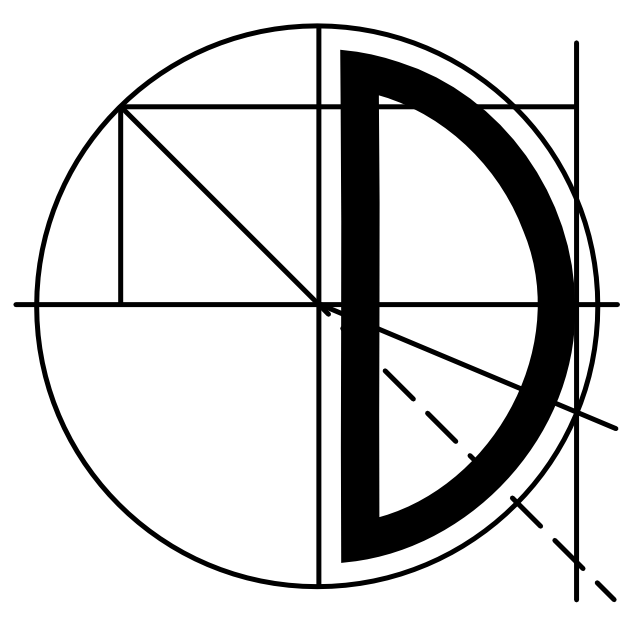
\includegraphics[width=\textwidth]{logos/DescartesSymbol_gross.png}
		\caption{Symbol placed on the left side.}
		\label{fig:descartessymbol1}
	\end{subfigure}
	\hfill
	\begin{subfigure}[b]{0.3\textwidth}
		\centering
		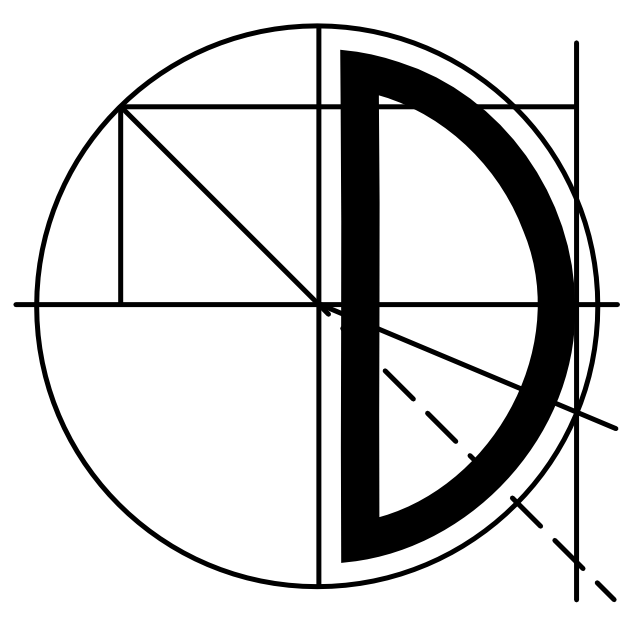
\includegraphics[width=\textwidth]{logos/DescartesSymbol_gross.png}
		\caption{Symbol placed in the middle.}
		\label{fig:descartessymbol2}
	\end{subfigure}
	\hfill
	\begin{subfigure}[b]{0.3\textwidth}
		\centering
		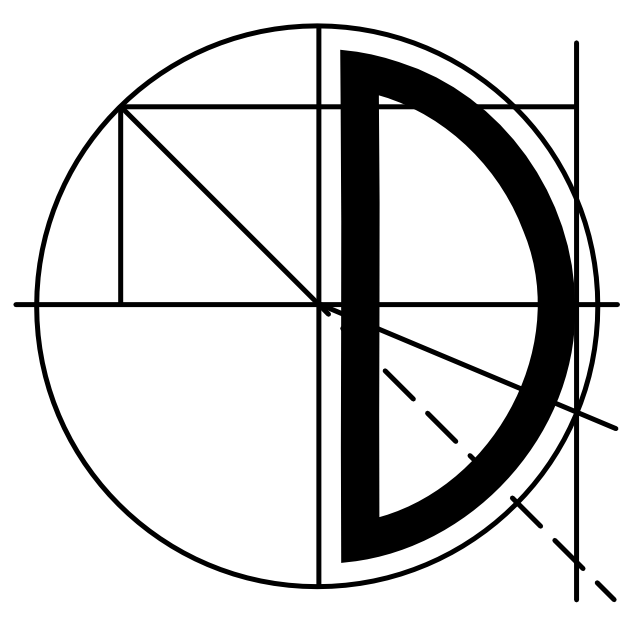
\includegraphics[width=\textwidth]{logos/DescartesSymbol_gross.png}
		\caption{Symbol placed on the right side.}
		\label{fig:descartessymbol3}
	\end{subfigure}
	\caption{Symbol of the Descartes research group.}
	\label{fig:descartessymbol}
\end{figure}

It is also possible to include \textit{.svg} figures via the \textit{svg} package, e.g.\ \verb|\includesvg{logos/example}|. This requires compiling with \verb|--shell-escape| and having \textit{Inkscape} installed locally. The resulting \textit{.pdf} is cached next to the source file.
\begin{figure}
%\includesvg{...}
\end{figure}


\section{Units}
To properly print units for measurements (e.g.\ time), use the \textit{siunitx} package.

Example: \qty{3}{\second} or \qty{8}{\milli\second} or \qty{222}{\kilo\metre\per\hour} or \qtyrange{10}{20}{\second} or \qty{10\pm 5}{\second}

Have a look at the \href{https://ctan.org/pkg/siunitx?lang=de}{package documentation} for more examples.

\section{ToDos}
Sometimes it may be worth, noting down a todo for later.\todo{This is a ToDo!}

You can later disable them by using \verb|\usepackage[disable]{todonotes}|.\todo{Don't forget to change that!}
However, you can also just delete them.
